\chapter{Implementação e testes}
\label{cap:implementacaoresultados}

Neste capítulo será descrito o ambiente de alta disponibilidade desenvolvida na empresa. Posteriormente será apresentada a metodologia de testes 
utilizada, bem como os resultados obtidos dos testes efetuados.

\section{Descrição do ambiente de alta disponibilidade}
\label{section:implementacao}

%Para implementação desta solução foram necessários dois servidores físicos, sendo que a configuração ideal de cada servidor é de 
%real = 11 \textit{cores} de processamento, 12 GB de memória \ac{RAM} e 156 GB de disco rígido
%12 \textit{cores} de processamento, 14 GB de memória \ac{RAM} e 180 GB de disco rígido. Essa configuração foi calculada a partir da soma dos 
%recursos das máquinas virtuais que atualmente abrangem os serviços que foram considerados críticos, observa-se que tais recursos de 
%\textit{hardware} já encontravam-se disponíveis, sendo necessário somente efetuar uma reorganização das máquinas virtuais. Com essa solução, 
%caso ocorra alguma falha em um servidor, as máquinas virtuais serão transferidas para o outro servidor.

O ambiente foi projetado na forma de um \textit{cluster}, o qual é composto por dois servidores com requisitos de configuração 
de 12 \textit{cores} de processamento, 14 GB de memória \ac{RAM} e 180 GB de disco rígido.
%real = 11 \textit{cores} de processamento, 12 GB de memória \ac{RAM} e 156 GB de disco rígido
Essa configuração foi calculada a partir da soma dos recursos consumidos pelas máquinas virtuais que anteriormente executavam os serviços que foram 
considerados críticos. Observa-se que tais recursos de \textit{hardware} já encontravam-se disponíveis, sendo necessário somente efetuar uma 
reorganização das máquinas virtuais. Destaca-se que a configuração também inclui 2 GB de memória \ac{RAM} e 24 GB de disco para cada sistema 
operacional hóspede.

Optou-se por utilizar o mesmo sistema operacional e o mesmo hipervisor que são utilizados na empresa, estes são, respectivamente, o sistema 
\textit{Ubuntu 14.04 \ac{LTS}} e o \ac{KVM} \cite{kvm}. O processo de instalação e de configuração encontra-se no 
Apêndice \ref{ap:confos} e \ref{ap:confvirt}.

\subsection{Estrutura física}

A estrutura física adotada encontra-se na Figura \ref{fig:projeto_fisico} (a). Como pode ser observado, os dois servidores encontram-se 
conectados a um \textit{switch} através de dois cabos \aca{UTP}, de forma a implementar uma redundância de cabeamento. Além disso, manteve-se o 
\textit{link aggregation} e utilizou-se uma \textit{bridge}\footnote[1]{\textit{Bridges}, também conhecidas como pontes, são meios que fazem a 
conexão entre \textit{LANs}, e operam na camada de enlace de dados.} para incluir as máquinas virtuais à rede dos servidores da empresa. 
Os detalhes da configuração de rede estão localizados no Apêndice \ref{ap:confrede}.
Na Figura \ref{fig:projeto_fisico} (b) tem-se a imagem dos servidores utilizados, sendo que o primeiro é o Nó 1 (\textit{Brina}), que é um 
\textit{Dell PowerEdge 2950}, e o segundo é o Nó 2 (\textit{Piova}), que é um \textit{Dell PowerEdge R410}.

\begin{figure}[h!]
 \centering
 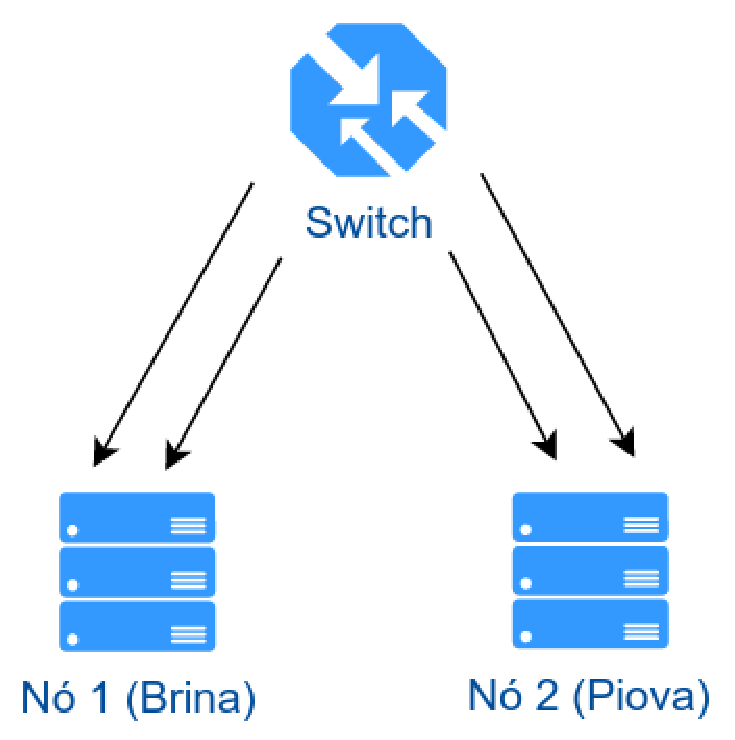
\includegraphics[width=430px]{img/projeto_fisico.eps}
 \caption{Estrutura física.}
 \label{fig:projeto_fisico}
\end{figure}

Imagem com drbd ??
descrição

\subsection{Estrutura lógica}

A estrutura lógica dos servidores juntamente com as máquinas virtuais e seus respectivos serviços são apresentados na Figura 
\ref{fig:projeto_estrutura}. Para a replicação de dados foi utilizado o \textit{software} \ac{DRBD}, que foi configurado no modo 
\textit{dual-master} onde os dois nós são configurados como primários. Para tal configuração foi necessário utilizar um sistema de arquivos 
distribuídos para um acesso compartilhado dos dados, sendo que o \textit{software} adotado foi o \ac{OCFS2} \cite{ocfs2}. 
Os detalhes da instalação e da configuração do \ac{DRBD} e do sistema de arquivos \ac{OCFS2} estão detalhadas no Apêndice \ref{ap:confdisco}. 

Já para o gerenciamento do \textit{cluster} e das \acp{VM} utilizou-se o \textit{software} \textit{Pacemaker}. 
Mais especificamente esse é o \textit{software} responsável pelo monitoramento e pela migração das \acp{VM} entre os nós.
Esse \textit{software} inicia e para os recursos de acordo com a configuração definida, por exemplo, ao iniciar o \textit{cluster} o 
\textit{Pacemaker} inicia o serviço de sincronismo do \ac{DRBD}, monta o sistema de arquivos no diretório onde está localizado os 
discos das \acp{VM}, e inicia as máquinas virtuais.

\begin{figure}[h!]
 \centering
 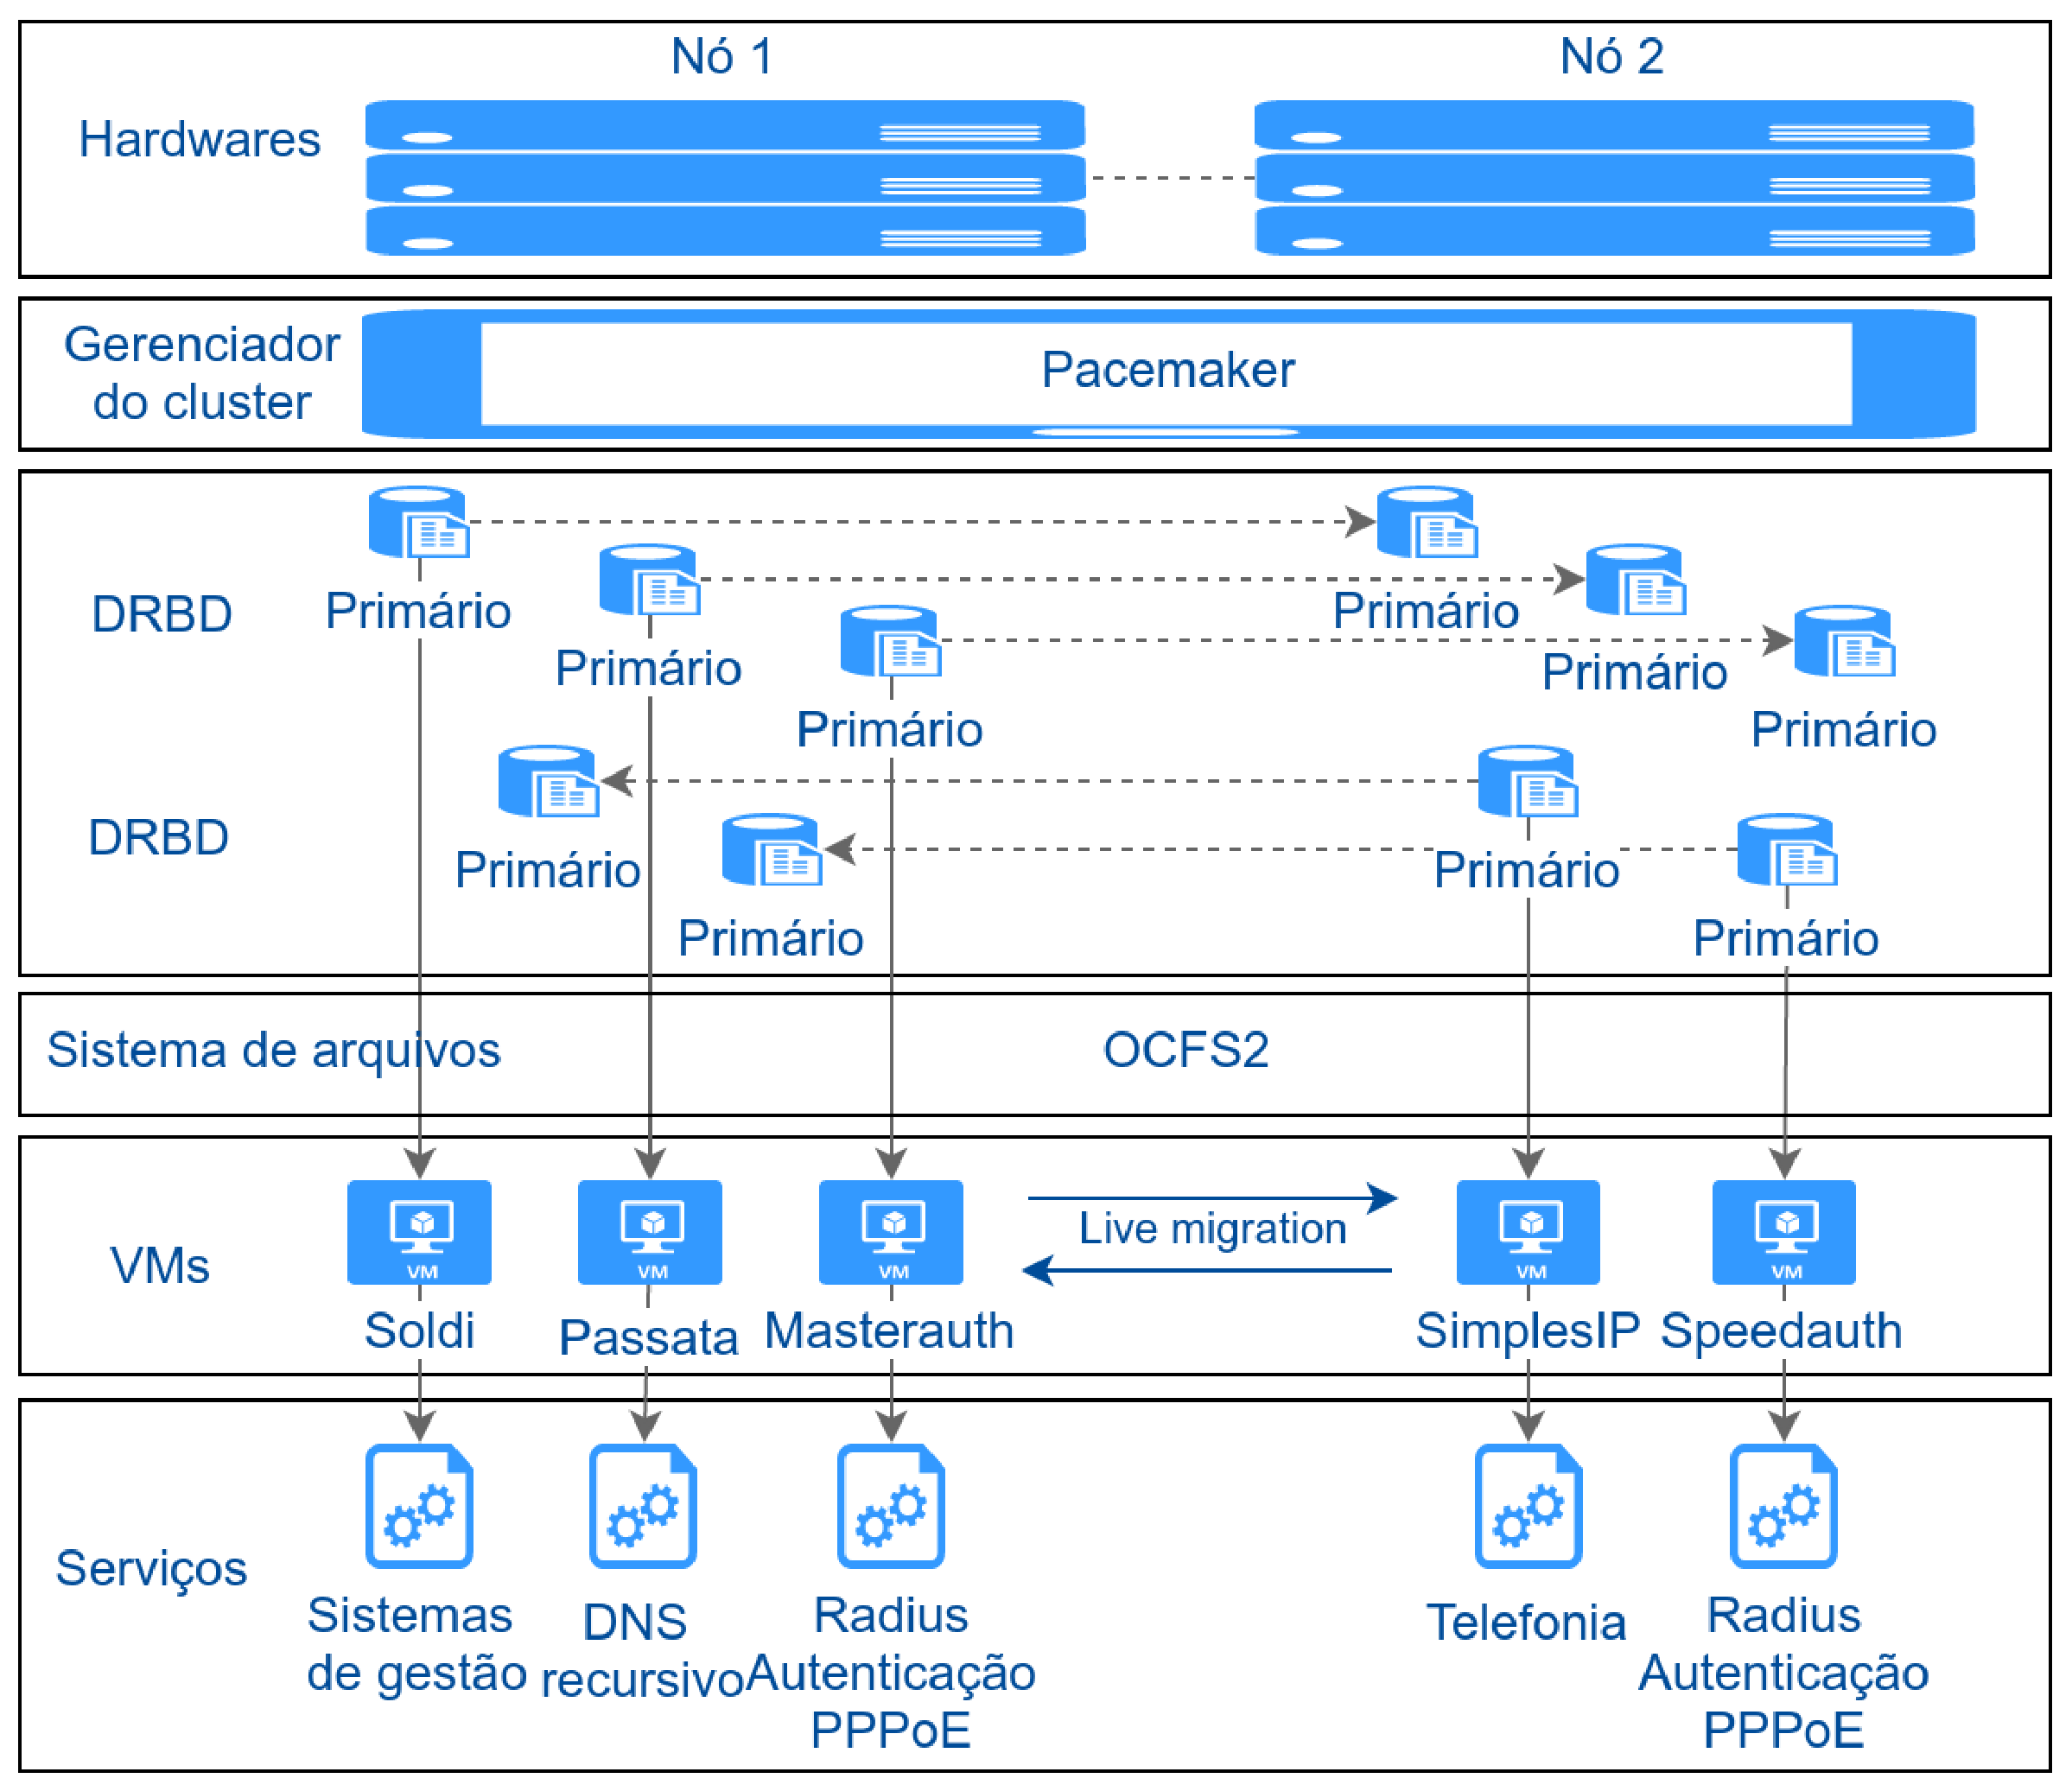
\includegraphics[width=350px]{img/projeto_estrutura.eps}
 \caption{Estrutura do \textit{cluster}.}
 \label{fig:projeto_estrutura}
\end{figure}

Os serviços foram distribuídos entre os nós do \textit{cluster}, sendo que no Nó 1 foram instalados os serviços de sistemas de gestão e 
autenticação \ac{PPPoE}. Já no Nó 2 foram instalados os serviços de \ac{DNS} recursivo, telefonia e autenticação \ac{PPPoE}.
No caso de falha em um nó, os serviços serão inicializados no outro nó disponível. O detalhamento da configuração do \textit{Pacemaker} 
estão disponíveis no Apêndice \ref{ap:confpacemaker}.

%drbd
% O \ac{DRBD} será configurado no modo \textit{master-slave}, sendo que para cada disco das máquinas virtuais será criado um dispositivo de 
% replicação \ac{DRBD}. E para utilizar esse dispositivo como disco de uma máquina virtual será criado um volume lógico 
% \ac{LVM}\footnote{LVM é uma ferramenta de código aberto que possibilita a manipulação de discos rígidos, através da criação de grupos de volumes 
% e volumes lógicos para \textit{Linux}.} \cite{lvm}. 


\section{Testes}

A metodologia de testes adotada neste trabalho foi baseada nos trabalhos de \citet{reis2009} e \citet{goncalves2009}. No primeiro trabalho, 
o autor simulou as falhas de três formas distintas, que foram através do desligamento brusco do servidor, desligamento por \textit{software} e 
falha de rede. Já no segundo trabalho, foram realizados três testes, que foram a reinicialização do servidor físico, a migração de uma 
máquina virtual de forma manual, e por fim um teste com migração em tempo real (\textit{live migration}).

Neste trabalho optou-se por utilizar o teste de desligamento brusco e o desligamento por \textit{software} que foram utilizados por 
\citet{reis2009}. Já de \citet{goncalves2009}, utilizou-se o teste de migração em tempo real, porém adaptado para simular um agendamento de 
manutenção de \textit{hardware} ou de \textit{software}.
%, ou seja, migrar as \acp{VM} de um nó para outro utilizando a migração em tempo real, 
%com objetivo de fazer uma manutenção do sistema operacional deste nó.

%Os três testes descritos nas próximas seções foram efetuados no ambiente de alta disponibilidade com uma máquina virtual para fins de experimento, 
%devido ao fato destes testes possuírem risco de perda de dados durante a execução.
%Todavia, na Seção \ref{section:comparacaofinal} será feita a medição e a análise do período de um mês no ambiente de alta disponibilidade,
%sendo que neste ambiente estarão executando os serviços críticos definidos.

\subsection{Teste 1 - Desligamento físico}
%Desligamento físico (simulação falha de hardware ou elétrica): 4 vezes para medir tempo de downtime dos serviços e dos nodes (serviço não crítico)

Neste teste são simuladas falhas de \textit{hardware} ou falhas elétricas nos nós do \textit{cluster}. Para isso foi feito o desligamento 
forçado de um servidor, ou seja, um servidor foi desligado de forma a simular a falha, sendo que os serviços devem ser transferidos de forma
automática para o outro servidor. Com esse teste pode-se avaliar o processo de \textit{failover} dos serviços (máquinas virtuais) que estavam 
executando no nó que falhou, bem como medir o tempo de indisponibilidade dos serviços. Esse teste foi executado 2 vezes em cada nó do 
\textit{cluster}. O tempo de indisponibilidade foi medido utilizando o comando \textit{ping} (para facilitar a medição foi utilizado um 
\textit{script} que encontra-se disponível no Apêndice \ref{ap:scriptindisp}), sendo que neste caso foi medido o tempo que o serviço ficou
fora do ar e tempo que o servidor físico permaneceu indisponível.

Na Tabela \ref{tab:teste1resultados} tem-se os resultados deste teste. Pode-se observar que o tempo de indisponibilidade do serviço 
(máquina virtual) é de apenas 81 segundos, isso se deve ao fato da \ac{VM} ser iniciada em um outro nó após o desligamento do primeiro. 
Caso um servidor de virtualização que não possua esta solução de alta disponibilidade, seja reiniciado por causa de uma falha elétrica por 
exemplo, o tempo para a recuperação do serviço seria igual a soma do tempo de inicialização do servidor físico mais o tempo de inicialização 
da máquina virtual, que totalizaria aproximadamente 250 segundos. 
Na pior das hipóteses, caso haja uma falha definitiva do servidor físico, sendo necessário reconfigurar a máquina virtual, reinstalar as aplicações,
configurá-las e restaurar o \textit{backup}, o \ac{MTTR} seria significativamente maior. Dependendo do servidor e da aplicação, 
a indisponibilidade poderia ser maior que 24 horas.
Pode-se observar na tabela uma diferença entre os tempos de indisponibilidade do Nó 1 e Nó 2, isso ocorre devido a utilização de \textit{hardwares}
diferentes na implementação. 
%Além disso, o desvio padrão demonstra que existe pouca variação entre os tempos de indisponibilidade.

%Este teste juntamente com os dois testes das próximas seções foram efetuados no 
%ambiente de alta disponibilidade com uma máquina virtual para fins de experimento, por possuírem risco de perda de dados em sua execução.

% feito em 15/09

\begin{table}[h!]
\caption{Resultados do teste de desligamento físico, contendo o tempo de indisponibilidade em segundos.}
\small
\label{tab:teste1resultados}
\begin{center}
\begin{tabular}{|l|l|}\hline
 & \textbf{Tempo de indisponibilidade médio} \\\hline % & \textbf{Desvio padrão da indisponibilidade} \\\hline
Nó 1 & 124 \\\hline % & 4,24 \\\hline
Nó 2 & 170,5 \\\hline % & 6,36 \\\hline
Máquina virtual & 81 \\\hline % & 7,07 \\\hline
\end{tabular}
\end{center}
\end{table}


%O procedimento deste teste é o seguinte:
%\begin{itemize}
% \item Acessar o terminal do servidor de monitoramento;
% \item Executar comando \textit{ping} e medir o tempo de indisponibilidade (\textit{script} no Apêndice \ref{ap:scriptindisp});
% \item Forçar desligamento do nó;
% \item Aguardar máquinas virtuais iniciarem no outro nó;
% \item Finalizar a medição do tempo e \textit{ping}.
%\end{itemize}

% A Figura \ref{fig:teste1_disponibilidade} demonstra a disponibilidade dos servidores físicos Nó 1 (\textit{Brina}) e Nó 2 (\textit{Piova}) e da 
% máquinas virtual (\textit{Trapel}). A máquina virtual teve apenas 1 minuto e 10 segundos de \textit{downtime}, deste modo, caso o 
% \textit{hardware} no qual a máquina virtual está executando falhe, o serviço será reestabelecido neste curto período de tempo.
% 
% \begin{figure}[h!]
%  \centering
%  \includegraphics[width=470px]{img/teste1_disponibilidade.eps}
%  \caption{Disponibilidade servidores físicos \textit{Brina} e \textit{Piova} e da máquina virtual \textit{Trapel}.}
%  \label{fig:teste1_disponibilidade}
% \end{figure}


\subsection{Teste 2 - Desligamento por software}

Esse teste simula falhas de \textit{software} nos nós do \textit{cluster}, sendo que neste caso pode-se citar como exemplo uma falha no 
\textit{software} de virtualização, com isso o nó não conseguiria iniciar a máquina virtual. Esse tipo de situação também pode ocorrer em uma 
falha de atualização do sistema operacional ou do \textit{kernel}, onde o sistema operacional do nó não conseguiria inicializar corretamente.
%Esse tipo de situação também pode ocorrer em uma manutenção emergencial, onde é preciso desligar um servidor físico de forma rápida. 
Neste tipo de falha os serviços devem ser transferidos para o outro nó de forma automática, assim reduzindo a indisponibilidade desses serviços. 
Desta forma, pode-se avaliar o processo de \textit{failover} dos serviços que estavam executando no nó que apresentou a falha.

Para simular esta falha, foram acessados os nós via \ac{SSH} e executado o comando \textit{reboot}.
Esse teste foi executado 2 vezes em cada um dos nós do \textit{cluster}. O tempo de indisponibilidade foi medido da mesma forma do que o teste 
anterior, utilizando o comando \textit{ping}. A medição desse tempo foi feita nos dois nós e também na máquina virtual. 
A Tabela \ref{tab:teste2resultados} apresenta o tempo de indisponibilidade dos nós e da \ac{VM}. 
Pode-se observar que o tempo de indisponibilidade da \ac{VM} é consideravelmente menor que o tempo do servidor físico. De fato, ele representa 
apenas 3,27\% do tempo de indisponibilidade dos servidores físicos que são 138,5 e 167 segundos. 

A alguns meses ocorreu um problema semelhante a este teste, um servidor de virtualização, que é atualizado de forma automática, foi reiniciado, 
porém ocorreu um erro na atualização e o servidor não inicializou corretamente. Os serviços executados nele ficaram aproximadamente 
6 horas indisponíveis.
% feito em 09/09

% O procedimento deste teste é o seguinte:
% \begin{itemize}
%  \item Acessar o terminal do servidor de monitoramento;
%  \item Executar comando \textit{ping} e medir o tempo de indisponibilidade (\textit{script} no Apêndice \ref{ap:scriptindisp});
%  \item Acessar o terminal do nó que será reiniciado;
%  \item Executar o comando \textit{reboot};
%  \item Aguardar máquinas virtuais iniciarem no outro nó e aguardar retorno do nó reiniciado;
%  \item Finalizar a medição do tempo e \textit{ping}.
% \end{itemize}

\begin{table}[h!]
\caption{Resultados do teste de desligamento por \textit{software}, com tempo de indisponibilidade em segundos.}
\small
\label{tab:teste2resultados}
\begin{center}
\begin{tabular}{|l|l|}\hline
 & \textbf{Tempo de indisponibilidade média} \\\hline % & \textbf{Desvio padrão da indisponibilidade} \\\hline
Nó 1 & 138,5 \\\hline % & 2,12 \\\hline
Nó 2 & 167 \\\hline % & 1,41 \\\hline
Máquina virtual & 10 \\\hline % & 0 \\\hline
\end{tabular}
\end{center}
\end{table}


\subsection{Teste 3 - Manutenção agendada}
%Agendamento de manutenção (reboot para atualização de software): 2 semanas ou mais, 1 manutenção por semana, com live migration, reboot e 
%atualização de kernel dos nodes. Resultados: latência, comparação downtime servidor virtual e físico, log

Reinicializações são necessárias para manutenções de \textit{hardware}, atualização de \textit{software} e até mesmo para 
rejuvenescimento\footnote{O rejuvenescimento de \textit{software} consiste na aplicações de métodos para remover problemas gerados pelo 
envelhecimento. Um exemplo de um método é o \textit{reboot} de um sistema operacional, uma vez que esse torna-se suscetível a gerar erros e 
falhas.} de \textit{software} \cite{melo2014}. Desta forma, criou-se esse teste para simular manutenções previamente agendadas.

%O procedimento deste teste é o seguinte:
%\begin{itemize}
% \item Executar comando \textit{ping} e medir o tempo de indisponibilidade (\textit{script} no Apêndice \ref{ap:scriptindisp});
% \item Executar o \textit{script} que desativa o nó (comando \textit{standby}) e executa o \textit{reboot} (Apêndice \ref{ap:scriptmanutencao});
% \item Após retorno do nó executar novamente o \textit{script} anterior para retorno do nó ao \textit{cluster};
% \item Finalizar a medição do tempo e \textit{ping}.
%\end{itemize}

Esse teste consiste no agendamento de 4 manutenções efetuadas durante o período de 13 dias, para tanto, criou-se um \textit{script} que é 
responsável por migrar as \acp{VM} de um nó e posteriormente reiniciá-lo, simulando assim uma atualização de \textit{kernel} 
(este \textit{script} está disponível no Apêndice \ref{ap:scriptmanutencao}). 
Para a execução do \textit{script} foi utilizada a ferramenta \textit{crontab} do \textit{Linux}. 

Na Tabela \ref{tab:teste3resultados} tem-se os resultados do teste. Como pode ser observado, o tempo de \textit{downtime} da máquina virtual 
é nulo, ou seja, não houve indisponibilidade nos serviços devido a migração em tempo real das \acp{VM}. 
Já nos nós  tem-se um tempo de indisponibilidade de 145,5 e 173 segundos devido a reinicialização destes.
%A latência baixa da máquina virtual demonstra que não há perda significante de desempenho durante a migração da máquina virtual de um nó para outro.

% feito em 17/09 a 30/09
% crontab brina:
% */10 04 * * 2 /usr/local/sbin/script_pacemaker_manutencao.sh
% crontab piova:
% */10 04 * * 4 /usr/local/sbin/script_pacemaker_manutencao.sh
% crontab monit:
%59 03 * * 2 cd /home/bruno/pacemaker/teste2/; bash indisponibilidade.sh 186.195.16.14 1
%59 03 * * 2 cd /home/bruno/pacemaker/teste2/; bash indisponibilidade.sh 186.195.16.13 1
%59 03 * * 4 cd /home/bruno/pacemaker/teste2/; bash indisponibilidade.sh 186.195.16.6 2
%59 03 * * 4 cd /home/bruno/pacemaker/teste2/; bash indisponibilidade.sh 186.195.16.13 2

\begin{table}[h!]
\caption{Resultados do teste de manutenção agendada, com o tempo de indisponibilidade em segundos e o desvio padrão.}
\small
\label{tab:teste3resultados}
\begin{center}
\begin{tabular}{|l|p{5.5cm}|p{5.5cm}|}\hline
 & \textbf{Tempo de indisponibilidade média} & \textbf{Desvio padrão da indisponibilidade} \\\hline
Nó 1 & 145,5 & 0,70 \\\hline
Nó 2 & 173 & 1,41 \\\hline
Máquina virtual & 0 & 0 \\\hline
\end{tabular}
\end{center}
\end{table}

A Tabela \ref{tab:teste3disp} demonstra o percentual de disponibilidade da \ac{VM} e dos nós do \textit{cluster} durante o período de 13 dias
do teste. Destaca-se que a máquina virtual não apresentou nenhuma indisponibilidade. 
Esses dados foram produzidos pela ferramenta \textit{Nagios} \cite{nagios}, que é responsável pelo monitoramento da empresa.

\begin{table}[h!]
\caption{Disponibilidade e tempo de indisponibilidade do período de 13 dias.}
\small
\label{tab:teste3disp}
\begin{center}
\begin{tabular}{|l|p{5.5cm}|p{5.5cm}|}\hline
 & \textbf{Disponibilidade} & \textbf{Tempo indisponibilidade} \\\hline
Nó 1 & 99,976\% & 4 minutos e 30 segundos \\\hline
Nó 2 & 99,975\% & 4 minutos e 40 segundos \\\hline
Máquina virtual & 100\% & 0 minutos \\\hline
\end{tabular}
\end{center}
\end{table}

%A Figura \ref{fig:teste2_trapel1} demonstra a disponibilidade da máquina virtual, onde pode-se perceber que não houve nenhuma indisponibilidade. 
%Esses dados foram produzidos pela ferramenta \textit{Nagios} \cite{nagios}, que faz o monitoramento da empresa. 
%gráfico comparativo nagios da disponibilidade do servidor fisico e do virtual
%gráfico nagios - Trends(gráfico) ou Availability (resumo) - Hosts - servidor - tempo 18/09 a 30/09 + Include Soft States = yes
% \begin{figure}[h!]
%  \centering
%  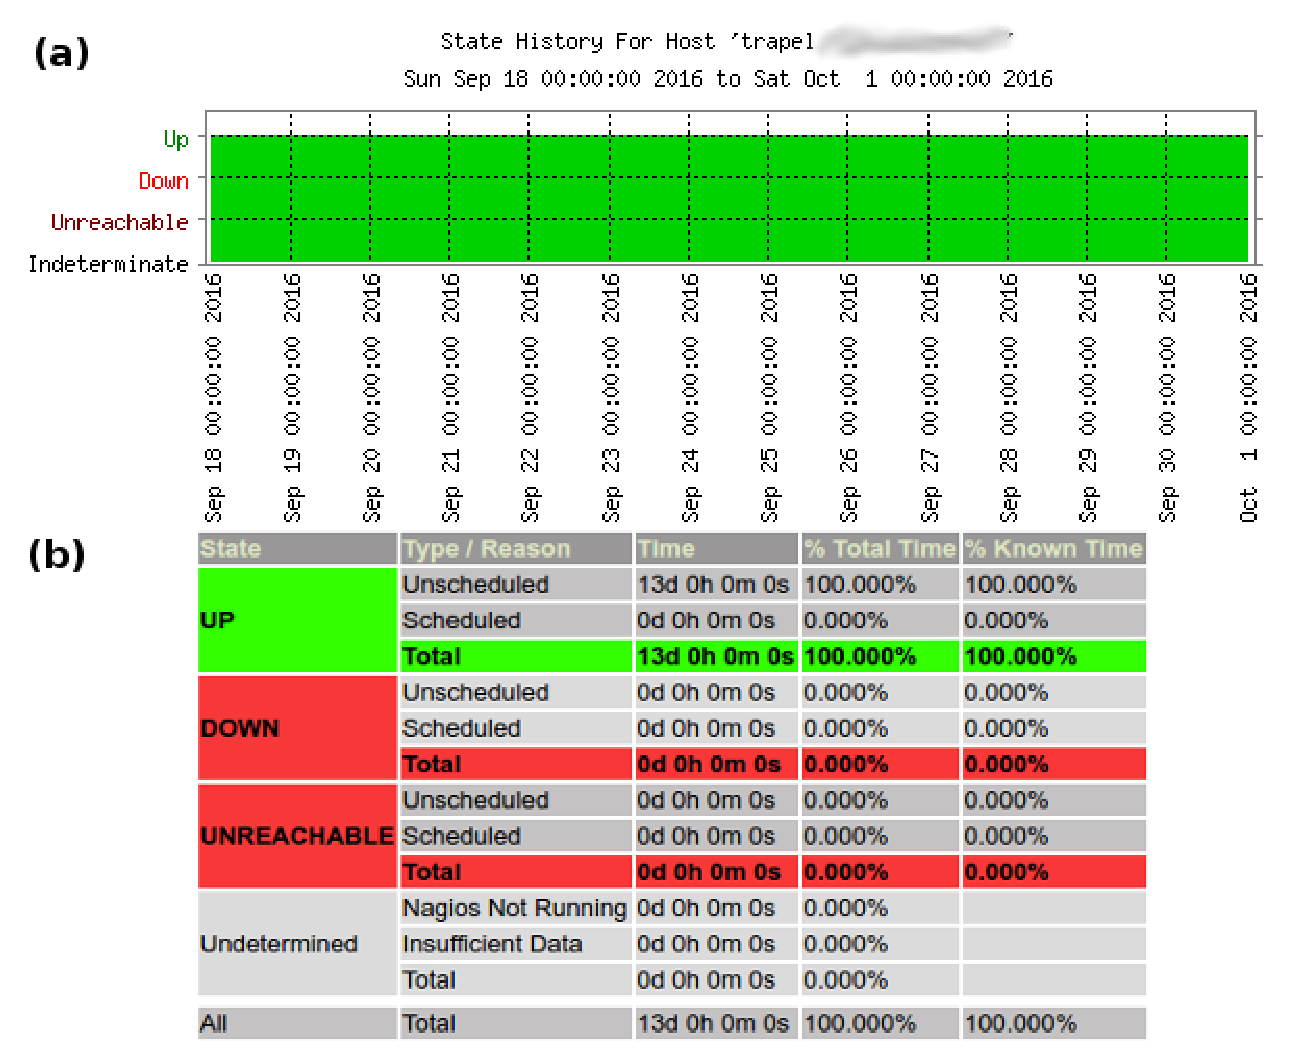
\includegraphics[width=360px]{img/teste2_trapel1.eps}
%  \caption{Disponibilidade da máquina virtual, com o gráfico da disponibilidade (a) e a tabela com detalhes de tempo e percentual (b).}
%  \label{fig:teste2_trapel1}
% \end{figure}

%Comparando os resultados da máquina virtual (Figura \ref{fig:teste2_trapel1} (b)) com os resultados dos nós 1 e 2 (Figura \ref{fig:teste2_brina1} 
%(b) e Figura \ref{fig:teste2_piova1} (b)), pode-se perceber a diferença do \textit{uptime}, que fica entre 99,975\% e 99,976\% para os nós e 
%100\% para a máquina virtual. Já nos gráficos da Figura \ref{fig:teste2_brina1} (a) e da Figura \ref{fig:teste2_piova1} (a), pode-se observar 
%as duas reinicializações feitas.
% \begin{figure}[h!]
%  \centering
%  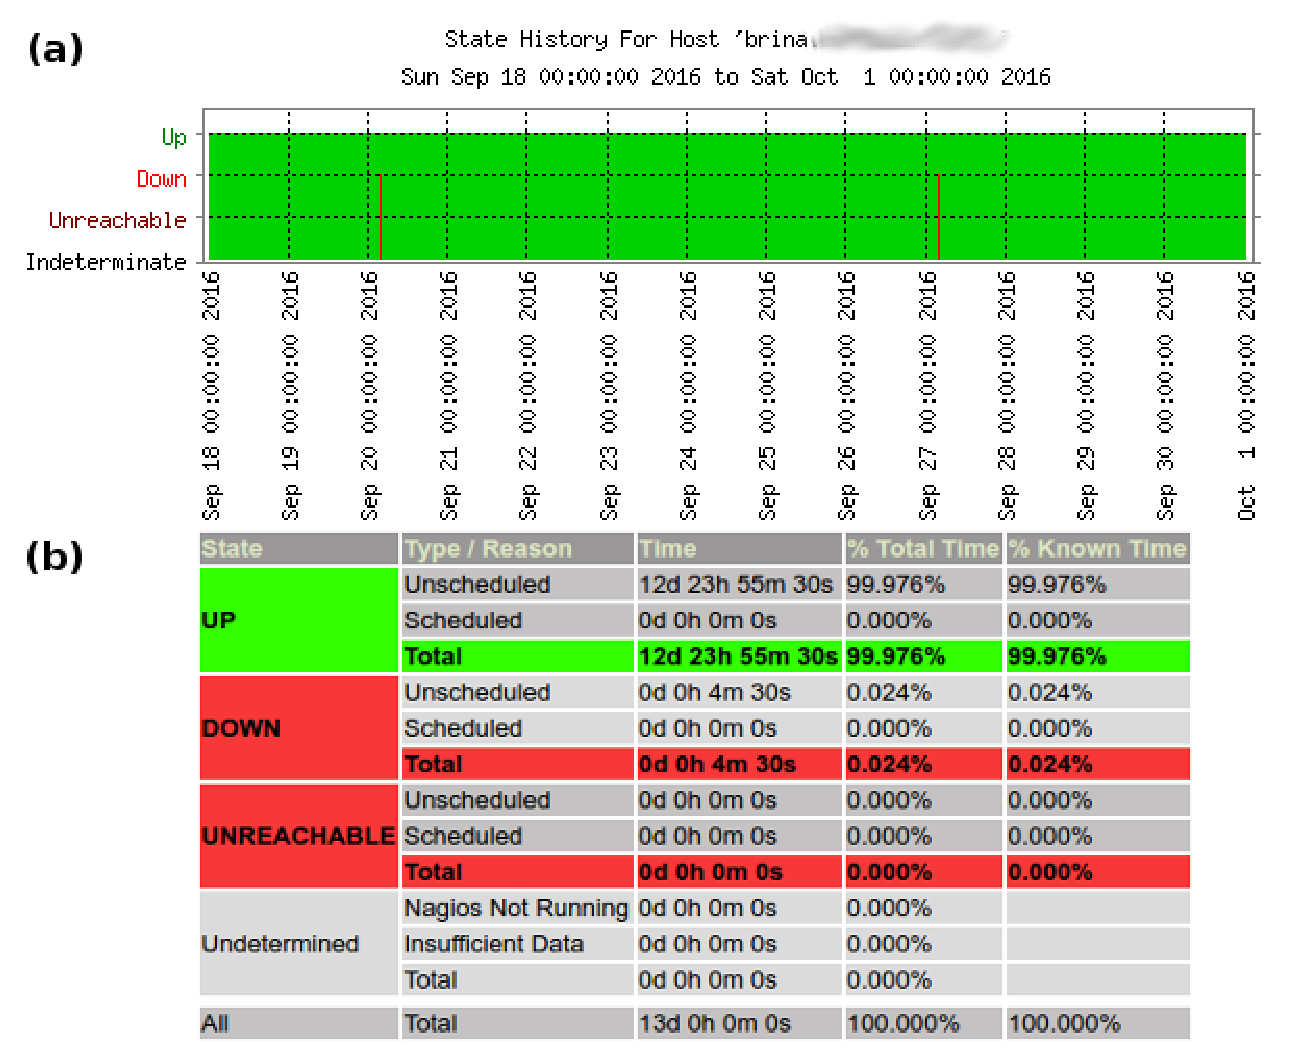
\includegraphics[width=360px]{img/teste2_brina1.eps}
%  \caption{Disponibilidade do Nó 1, com o gráfico da disponibilidade (a) e a tabela com detalhes de tempo e percentual (b).}
%  \label{fig:teste2_brina1}
% \end{figure}
% 
% \begin{figure}[h!]
%  \centering
%  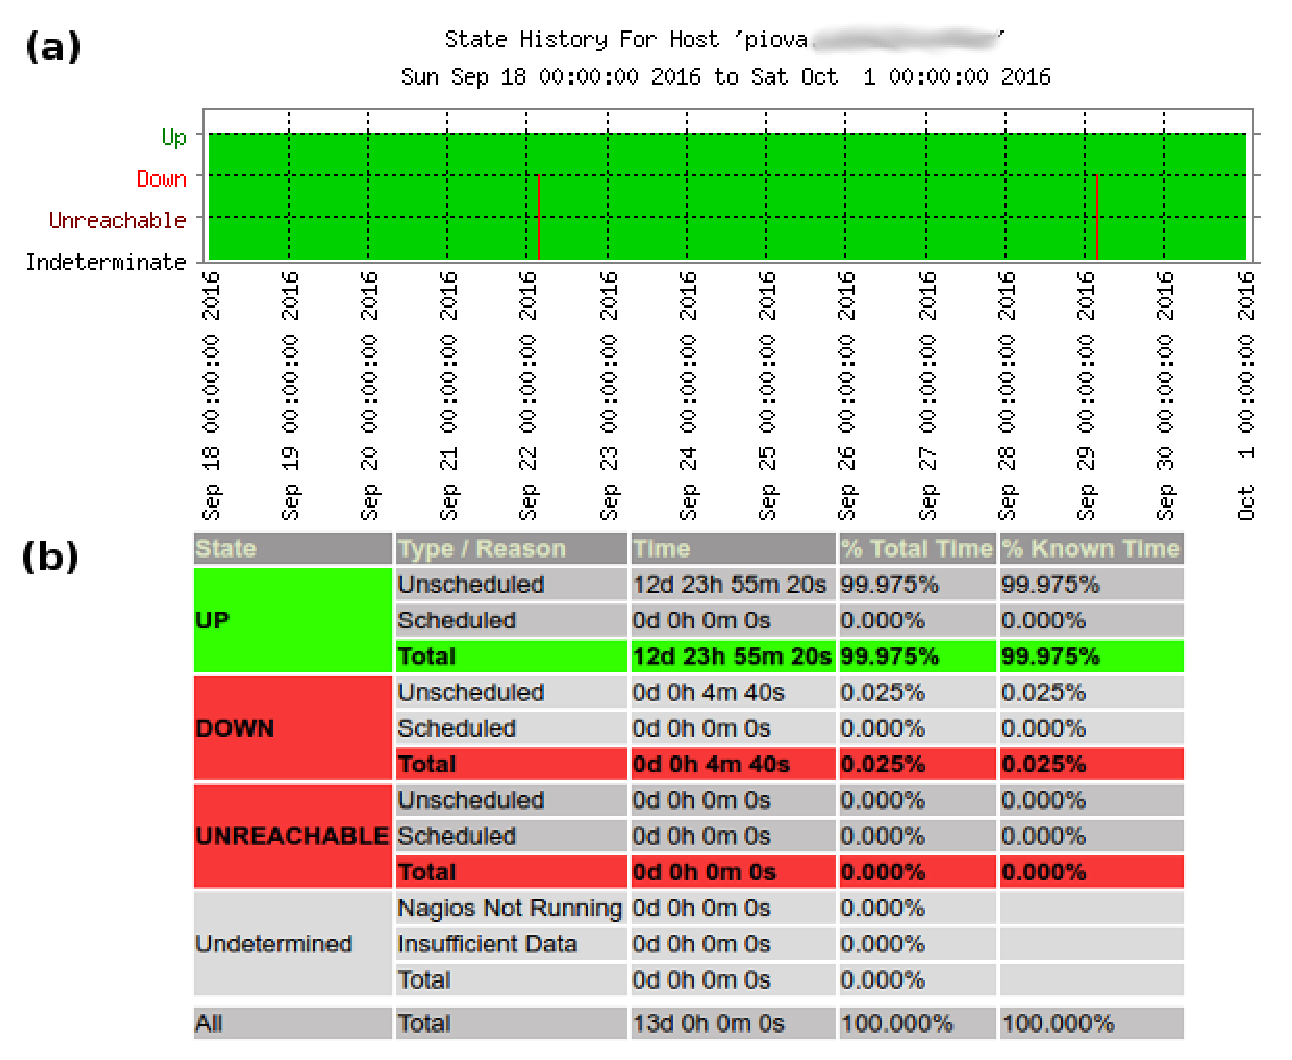
\includegraphics[width=360px]{img/teste2_piova1.eps}
%  \caption{Disponibilidade do Nó 2, com o gráfico da disponibilidade (a) e a tabela com detalhes de tempo e percentual (b).}
%  \label{fig:teste2_piova1}
% \end{figure}

Durante o processo de \textit{live migration} de um nó para outro a latência da máquina virtual aumentou\footnote[1]{
O aumento de latência deve-se ao fato da memória e os dados necessários para a migração da máquina virtual serem transferidos através da rede.}, 
isso pode ser observado na Figura \ref{fig:teste2_latencia}, onde tem-se um pico no intervalo de tempo de 50 à 100 segundos.
%Mesmo com o aumento de latência não ocorre perda significante de desempenho durante a migração da máquina virtual.
%teste2/186.195.16.13-stat-1.log
%teste2/186.195.16.13-stat-2.log
\begin{figure}[h!]
 \centering
 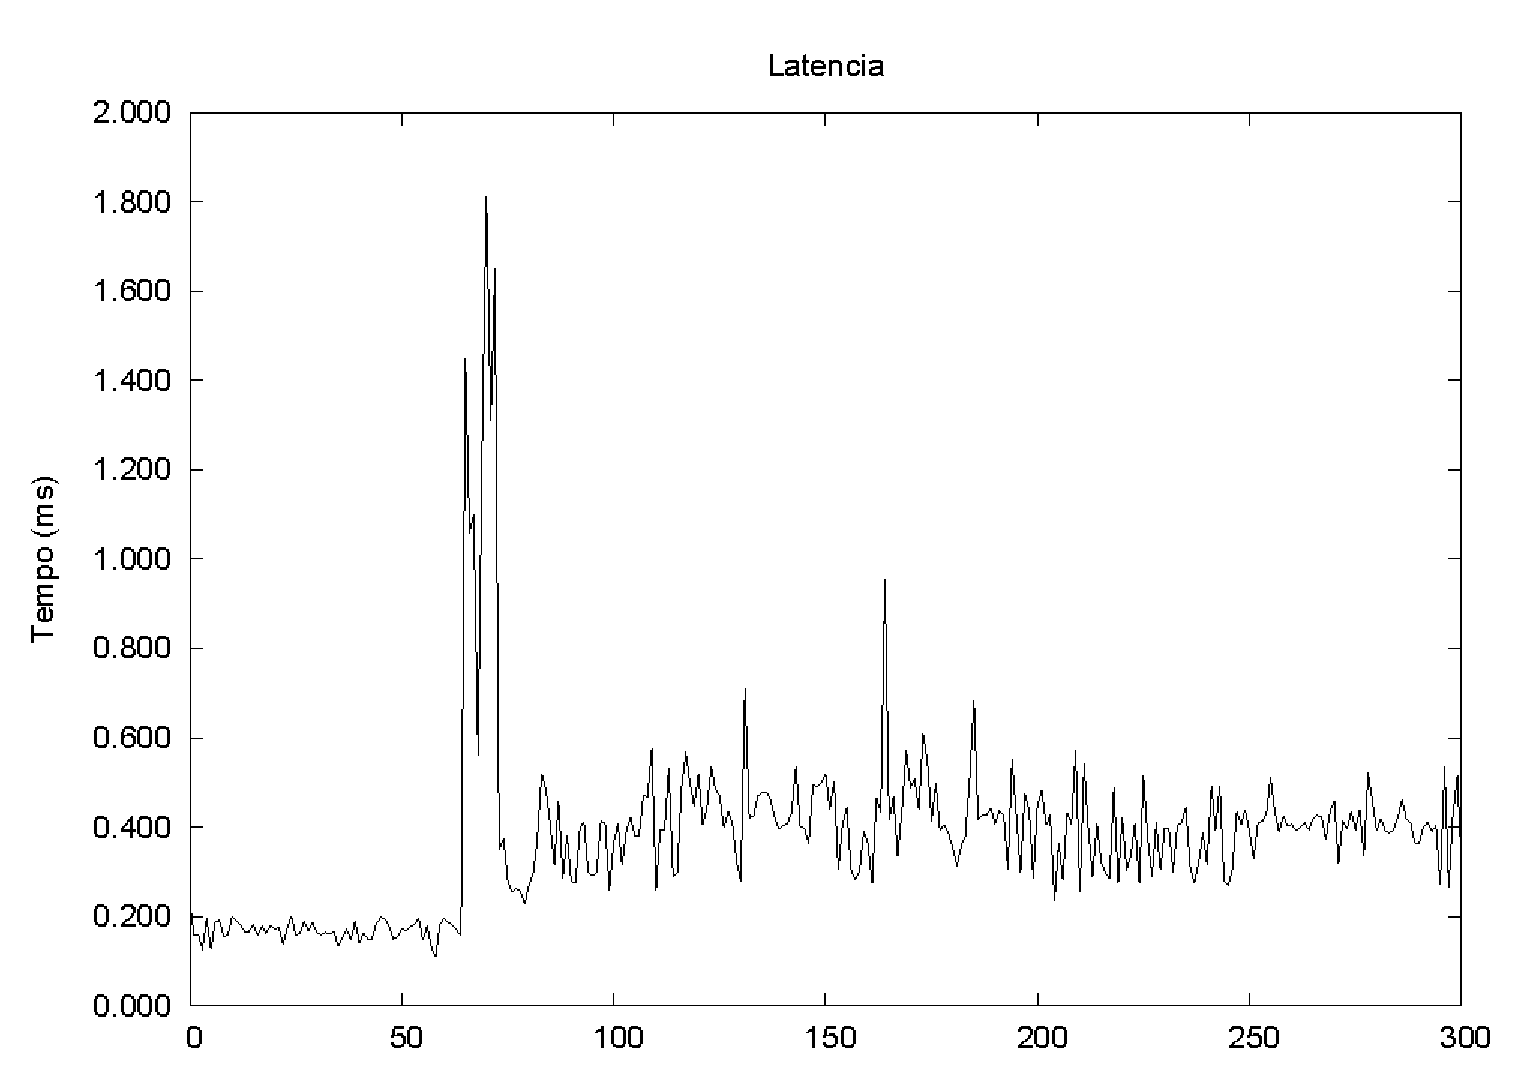
\includegraphics[width=320px]{img/teste2_latencia.eps}
 \caption{Latência da máquina virtual durante o \textit{live migration}.}
 \label{fig:teste2_latencia}
\end{figure}

%log do pacemaker
%O processo de \textit{standby} feito pelo \textit{Pacemaker} está detalhado no \textit{log} abaixo:


\section{Comparação final da disponibilidade}
\label{section:comparacaofinal}
%Medição da disponibilidade dos serviços críticos por 30 dias (14/10 a 12/11) FAZER uma manutenção de hardware.
%Comparar ao mês de setembro (01/09 a 30/09) no ambiente antigo com uma reinicialização dos servidores físicos (reiniciados em 06/09/16)

Esta última seção tem como objetivo comparar e analisar a disponibilidade do ambiente antigo com o ambiente de alta disponibilidade que foi 
implementado. Sendo assim foi feita uma medição da disponibilidade do período de um mês no ambiente antigo e de um mês no ambiente de alta 
disponibilidade implementado, sendo que nestes ambientes encontravam-se executando os serviços críticos que foram definidos na 
Seção \ref{section:maqservcrit}. Destaca-se que durante esses períodos foram feitas reinicializações nos servidores físicos, para atualização de
\textit{kernel}.

A Tabela \ref{tab:testefinal} apresenta a disponibilidade de cada máquina virtual com seu respectivo serviço no ambiente antigo e no 
ambiente de alta disponibilidade que foi criado. Pode-se observar que a disponibilidade máxima dos serviços no antigo ambiente é de apenas três 
noves, já no ambiente de alta disponibilidade tem-se uma disponibilidade próxima a 100\%.

%graficos: nagios_disponibilidade1_*
\begin{table}[h!]
\caption{Disponibilidade do antigo ambiente e do novo ambiente de alta disponibilidade, que foram medidos no período de um mês.}
\small
\label{tab:testefinal}
\begin{center}
\begin{tabular}{|l|l|p{4cm}|p{4cm}|}\hline
\textbf{Servidor} & \textbf{Serviço} & \textbf{Disponibilidade do antigo ambiente} & \textbf{Disponibilidade do novo ambiente} \\\hline
Passata & DNS recursivo & 99,978\% & 99,996\% \\\hline
Speedauth & Autenticação \ac{PPPoE} & 99,936\% & 100\% \\\hline
Masterauth & Autenticação \ac{PPPoE} & 99,930\% & 100\% \\\hline
Soldi & Sistemas & 99,913\% & 100\% \\\hline
SimplesIP & Telefonia & 99,866\% & 100\% \\\hline
\end{tabular}
\end{center}
\end{table}

A Tabela \ref{tab:testefinal2} demonstra o tempo de indisponibilidade de cada serviço, observa-se que o ambiente de alta disponibilidade
criado não apresentou indisponibilidade com exceção do serviço de \ac{DNS}, este 1 minuto e 40 segundos de indisponibilidade ocorreu devido 
a um problema de segurança que ocorreu durante o período de medição dos dados.

\begin{table}[h!]
\caption{Tempo de indisponibilidade dos serviços críticos nas dois ambientes.}
\small
\label{tab:testefinal2}
\begin{center}
\begin{tabular}{|l|l|p{4cm}|p{4cm}|}\hline
\textbf{Servidor} & \textbf{Serviço} & \textbf{Tempo de indisponibilidade do antigo ambiente} & \textbf{Tempo de indisponibilidade do novo ambiente} \\\hline
Passata & DNS recursivo & 9 minutos 40 segundos & 1 minuto 40 segundos \\\hline
Speedauth & Autenticação \ac{PPPoE} & 27 minutos 40 segundos & 0 \\\hline
Masterauth & Autenticação \ac{PPPoE} & 30 minutos 20 segundos & 0 \\\hline
Soldi & Sistemas & 37 minutos 20 segundos & 0 \\\hline
SimplesIP & Telefonia & 58 minutos 0 segundos & 0 \\\hline
\end{tabular}
\end{center}
\end{table}


\section{Considerações finais}

Neste capítulo foi apresentada a arquitetura de alta disponibilidade implementada com base em virtualização, sendo composta por dois servidores 
físicos, onde foram configuradas máquinas virtuais contendo os serviços críticos da empresa. Além disso, utilizou-se ferramentas de gerenciamento 
de \textit{cluster} e de replicação de dados para permitir a implementação da alta disponibilidade.

Foi feita uma análise do ambiente de alta disponibilidade implementado na empresa, através de testes e da coleta de dados provenientes desses. 
Para possibilitar a medição dos dados de disponibilidade foi utilizado \textit{scripts} e o comando \textit{ping}, além da ferramenta de 
monitoramento da empresa (\textit{Nagios}). Com o tempo de indisponibilidade do antigo ambiente e do ambiente de alta disponibilidade criado,
pôde-se comparar esses dois ambientes.
Com isso pode-se concluir que resultados obtidos foram positivos, e que os objetivos deste trabalho foram alcançados. 

